\documentclass{beamer}
\mode<presentation>{\usetheme{AV}}
\usepackage{etex}
\usepackage[export]{adjustbox}
\usepackage{epsfig}
\usepackage{feynmp}
\usepackage{verbatim}
\usepackage{listings}
\usepackage{colortbl}

\usepackage{color}

\definecolor{mygreen}{rgb}{0,0.6,0}
\definecolor{mygray}{rgb}{0.5,0.5,0.5}
\definecolor{mymauve}{rgb}{0.58,0,0.82}


\usepackage[utf8]{inputenc}
\usepackage[T1]{fontenc}
\usepackage{lmodern}
\usepackage{amsfonts}
\usepackage{supertabular}

\usepackage{textcomp}
\usepackage{amsmath}
\usepackage{amssymb}
\usepackage{graphicx}
%\usepackage{wrapfig}
\usepackage{subfigure}
\usepackage{type1cm}
\usepackage{tikz}
\usepackage{tikz-3dplot}
\usepackage{tikz}
\usepackage{tikz-3dplot}
\usepackage{pgfplots}
\usepackage{ulem}
\usetikzlibrary{shapes,arrows}
\usepackage{pgfplots}
\usetikzlibrary{shapes,arrows}
\usepackage{rotating}%     - to rotate boxes, pictures etc.
\usepackage{amsmath}%      - to use the AMS extended math package
\usepackage{amssymb}%      - to obtain additional math symbols in AMS fonts
\usepackage{amscd}%        - to obtain AMS flow chart utilities
\usepackage{array}%        - to obtain additional tabular functionality
\usepackage{multirow}%     - for multirow-entries in tables
\usepackage{supertabular}% - for multi-page tables
\usepackage{dcolumn}%      - decimal-point aligned colums in tables
\usepackage{xspace}%       - to add empty space after commands
\usepackage{upgreek}%      - provide upright greek letters
\usepackage{calc}%         - enhanced calculus in LaTeX macros
\usepackage{ifthen}%       - enhance logical structures in LaTeX macros
\usepackage{cite}%         - for multiple citations like [1-4] instead of [1,2,3,4]
\usepackage{tikz} 
%\usepackage{enumitem} 
\usepackage{multirow}
\usepackage{amssymb}
\usepackage{mathtools}
\usepackage{graphicx}
%\usepackage[dvipsnames]{xcolor}
%\input{../JADESEC-def}










%\setbeamertemplate{navigation symbols}{}
%\setbeamertemplate{footline}[page number]{}


%\newenvironment{changemargin}[2]{%
%\begin{list}{}{%
%\setlength{\topsep}{0pt}%
%\setlength{\leftmargin}{#1}%
%\setlength{\rightmargin}{#2}%
%\setlength{\listparindent}{\parindent}%
%\setlength{\itemindent}{\parindent}%
%\setlength{\parsep}{\parskip}%
%}%
%\item[]}{\end{list}}

%\newcommand{\maxFrameImage}[1]{
%\begin{frame}[plain]
%\begin{changemargin}{-1cm}{-1cm}
%\begin{center}
%\includegraphics[width=1.0\paperwidth,height=1.0\paperheight,keepaspectratio]
%{#1}
%\end{center}
%\end{changemargin}
%\end{frame}
%}


\def\Tiny{\fontsize{4.0pt}{4.0pt}\selectfont}

\title[DPHEP2017]{2nd DPHEP Collaboration Meeting}
\subtitle[DPHEP2017]{DPHEP2017}
\author[Andrii Verbytskyi]{
Andrii Verbytskyi
}
\date[]{\\ \today}


\setbeamersize{text margin left=.3cm,text margin right=.3cm} 
\listfiles
\begin{document}

\usebackgroundtemplate{%
  \tikz\node [anchor=north east, inner sep=0pt,opacity=0.18]  at (current page.center)
     {\includegraphics[height=0.5\paperheight,width=\paperwidth]{bkg3.eps}};
}

\frame{
%  \node [anchor=north east, inner sep=0pt,opacity=0.18]  at (current page.center)
 %    {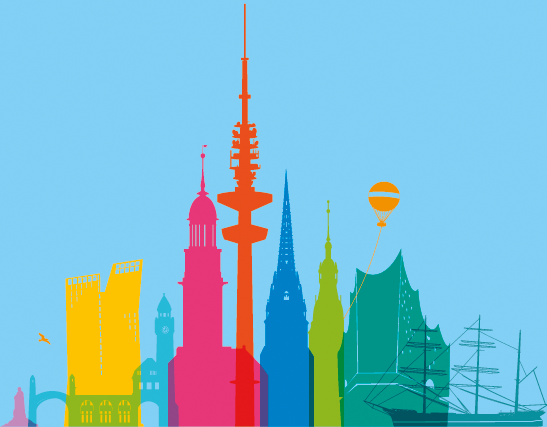
\includegraphics[height=0.097\paperheight,width=0.5\paperwidth]{bg}};
     
     %\begin{tikzpicture}%[remember picture, overlay]
%\end{tikzpicture}          
\vspace{0.3cm}
\begin{figure}
%\includegraphics[height=1.0cm]{eps/jade.eps}

\includegraphics[height=1.0cm]{eps/MPP_os_logo_cmyk.eps}

\includegraphics[height=1.0cm]{eps/DESY-Logo-cyan-RGB_ger.eps}
\hspace*{12.0cm}
\end{figure}
\begin{center}
\vspace{1.3cm}
{\LARGE The JADE long term data preservation projects in Max-Planck Institute f\"{u}r Physik}
\vspace{0.3cm}
\end{center}
\begin{center}
\vspace{0.3cm}
Andrii Verbytskyi on behalf of JADE Resurrection Group\\
\end{center}
\vspace{1.0cm}
\begin{center}
\footnotesize  2nd DPHEP Collaboration Meeting \\Geneva,\\ \today
\end{center}
\vspace{0.4cm}
}


\usebackgroundtemplate{%
  \tikz\node [anchor=north east, inner sep=0pt,opacity=0.98]  at (current page.center)
     {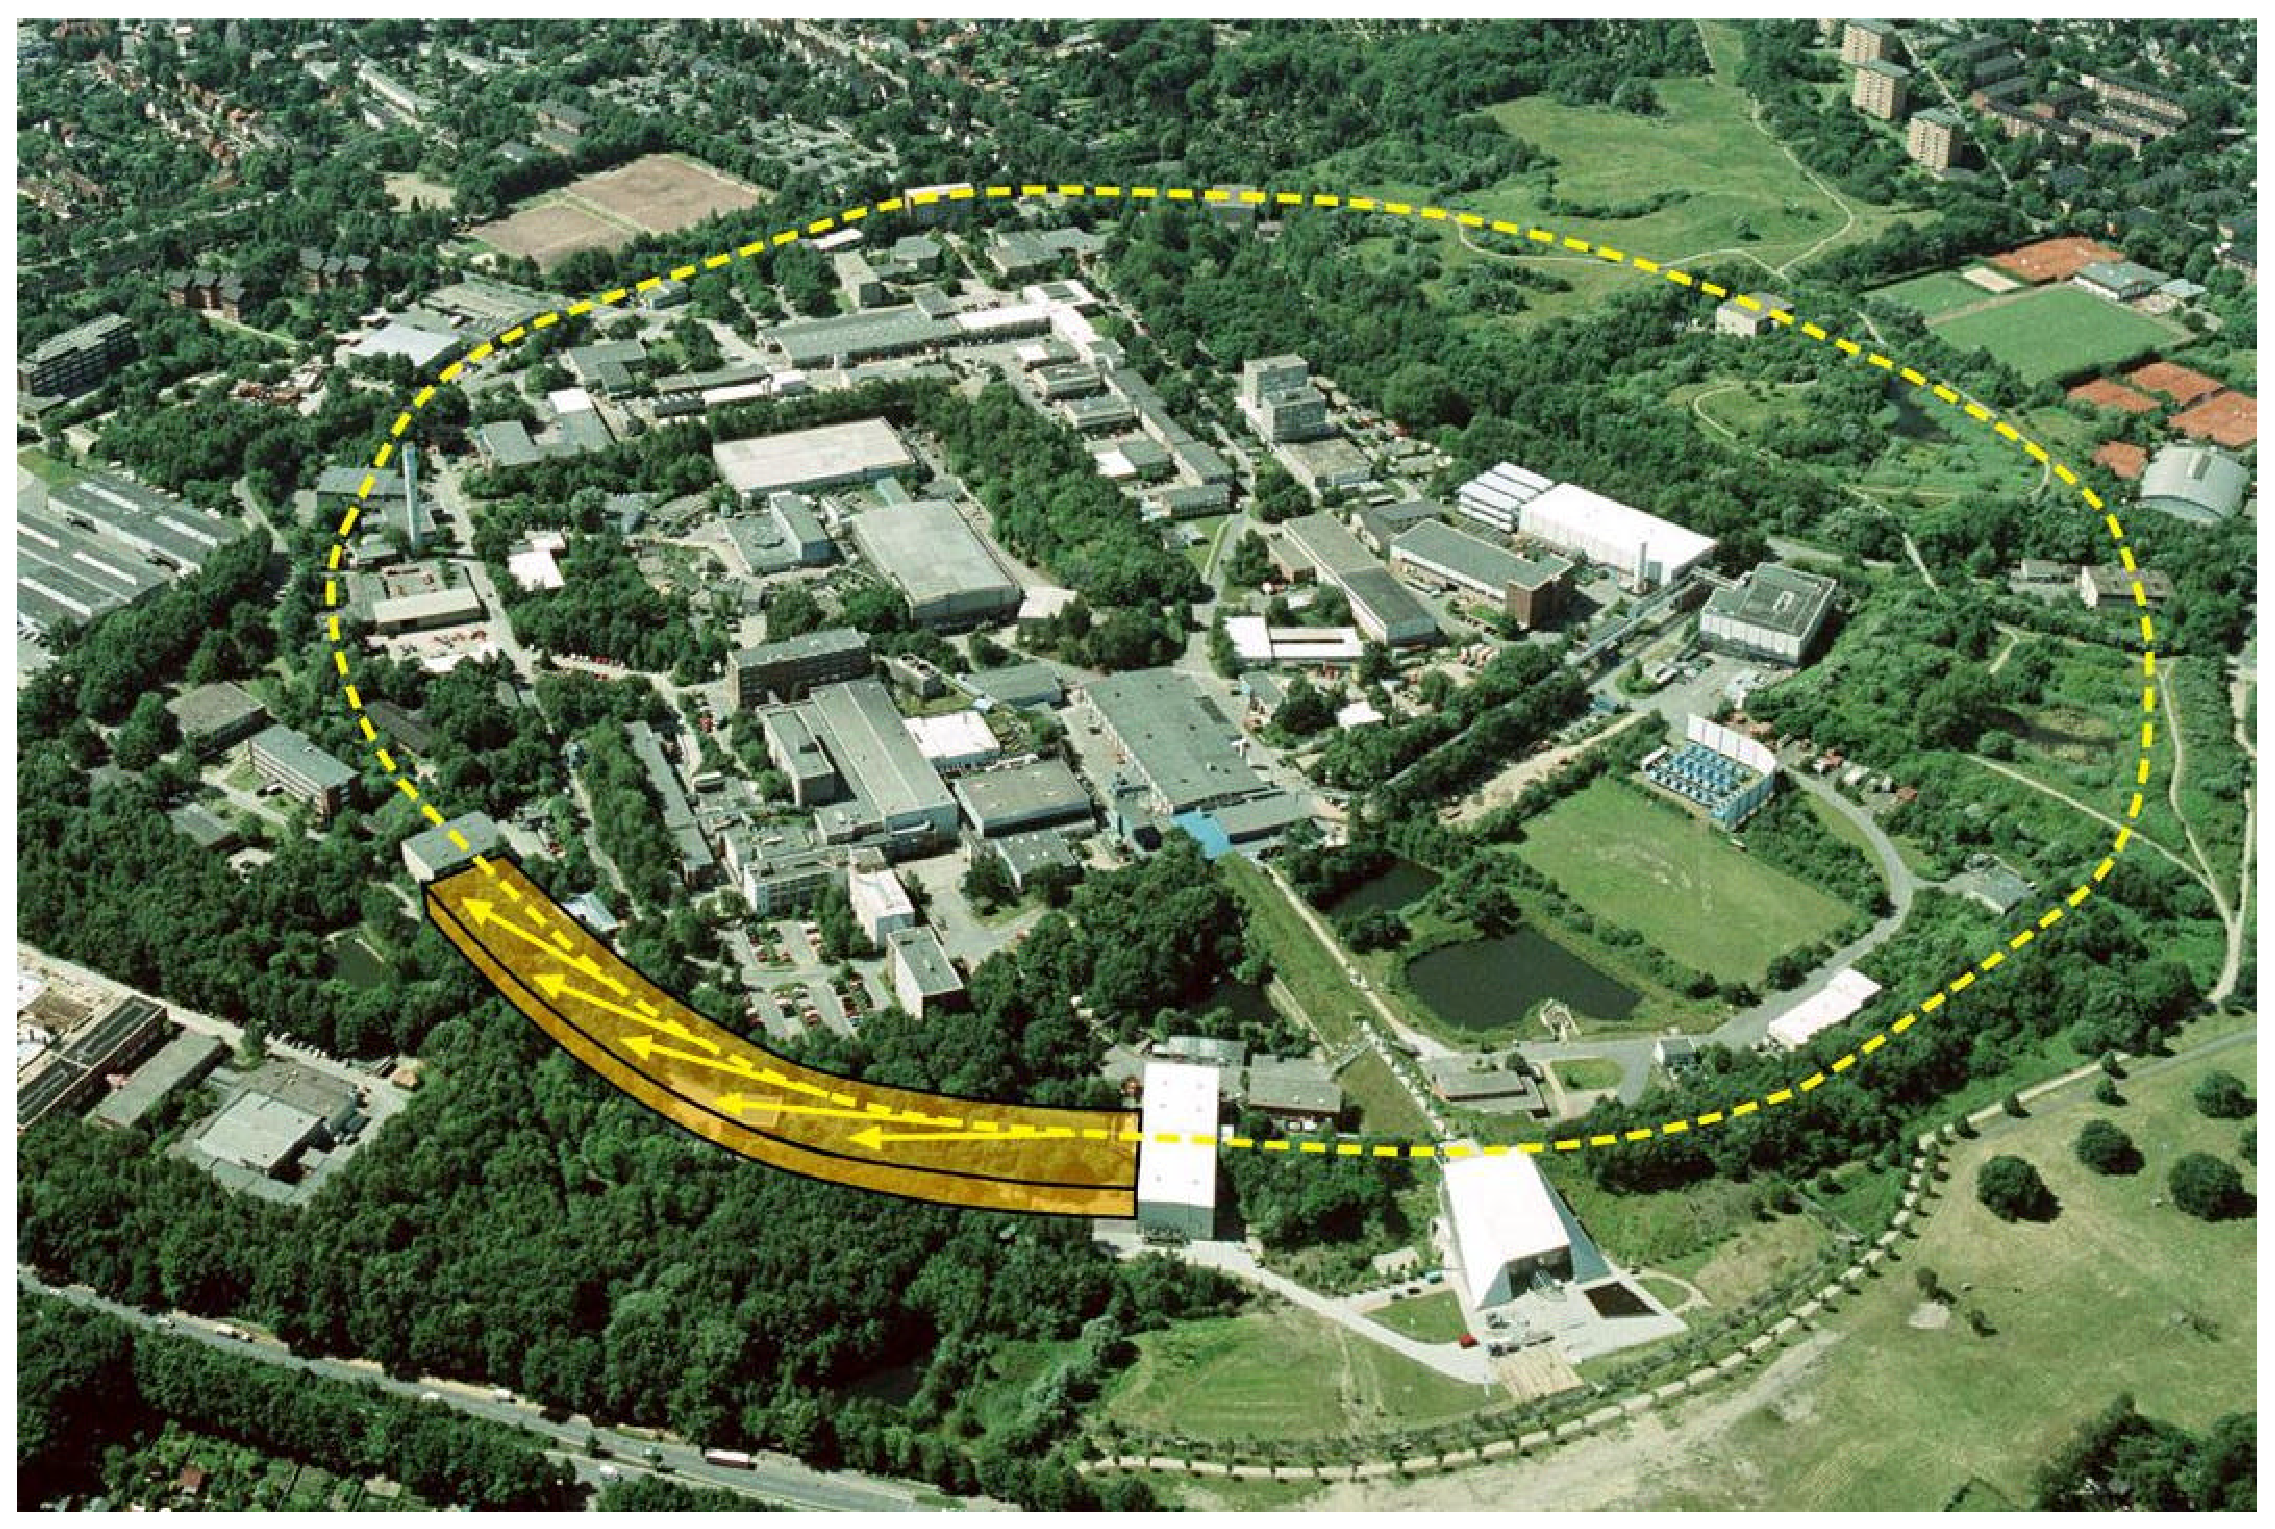
\includegraphics[height=1.0\paperheight,width=\paperwidth]{PETRA}};
}


\frame{\frametitle{PETRA}
{\color{white}\Large\bf 
\begin{itemize} 
\item \color{white} Electron-positron collider, started in 1979 in DESY; 
\item \color{white}2.3km ring, beam energies up to 23GeV;
\item \color{white}Experiments: TASSO, MARK-J, CELLO, {\color{red}JADE}.
\end{itemize} 
} 
}
\usebackgroundtemplate{}

\frame{\frametitle{JADE}
\begin{centering}
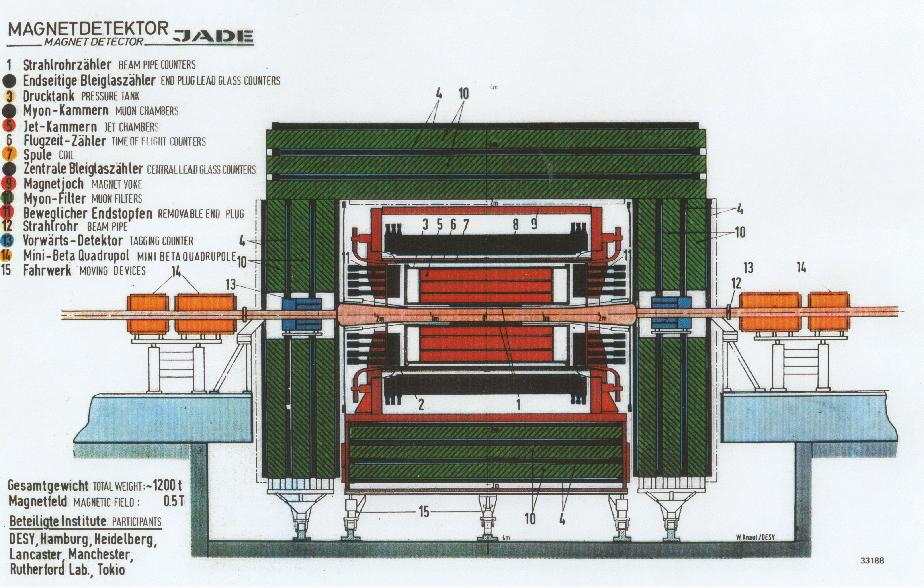
\includegraphics[width=0.8\linewidth]{eps/JADEDet.eps}	
\end{centering}
\begin{columns}[c]
\column{0.49\linewidth}
\begin{itemize} 
\item multipurpose detector 
\item large solid angle coverage
\item digital readout
\end{itemize} 
\column{0.49\linewidth}
\begin{itemize} 
\item advanced tracking system
\item calorimeter
\item muon chambers
\end{itemize} 
\end{columns}
{\bf \color{red} 35 years later: still unique energy range coverage!}
}


%eps/JADEDet.eps

\usebackgroundtemplate{%
  \tikz\node [anchor=north east, inner sep=0pt,opacity=0.18]  at (current page.center)
     {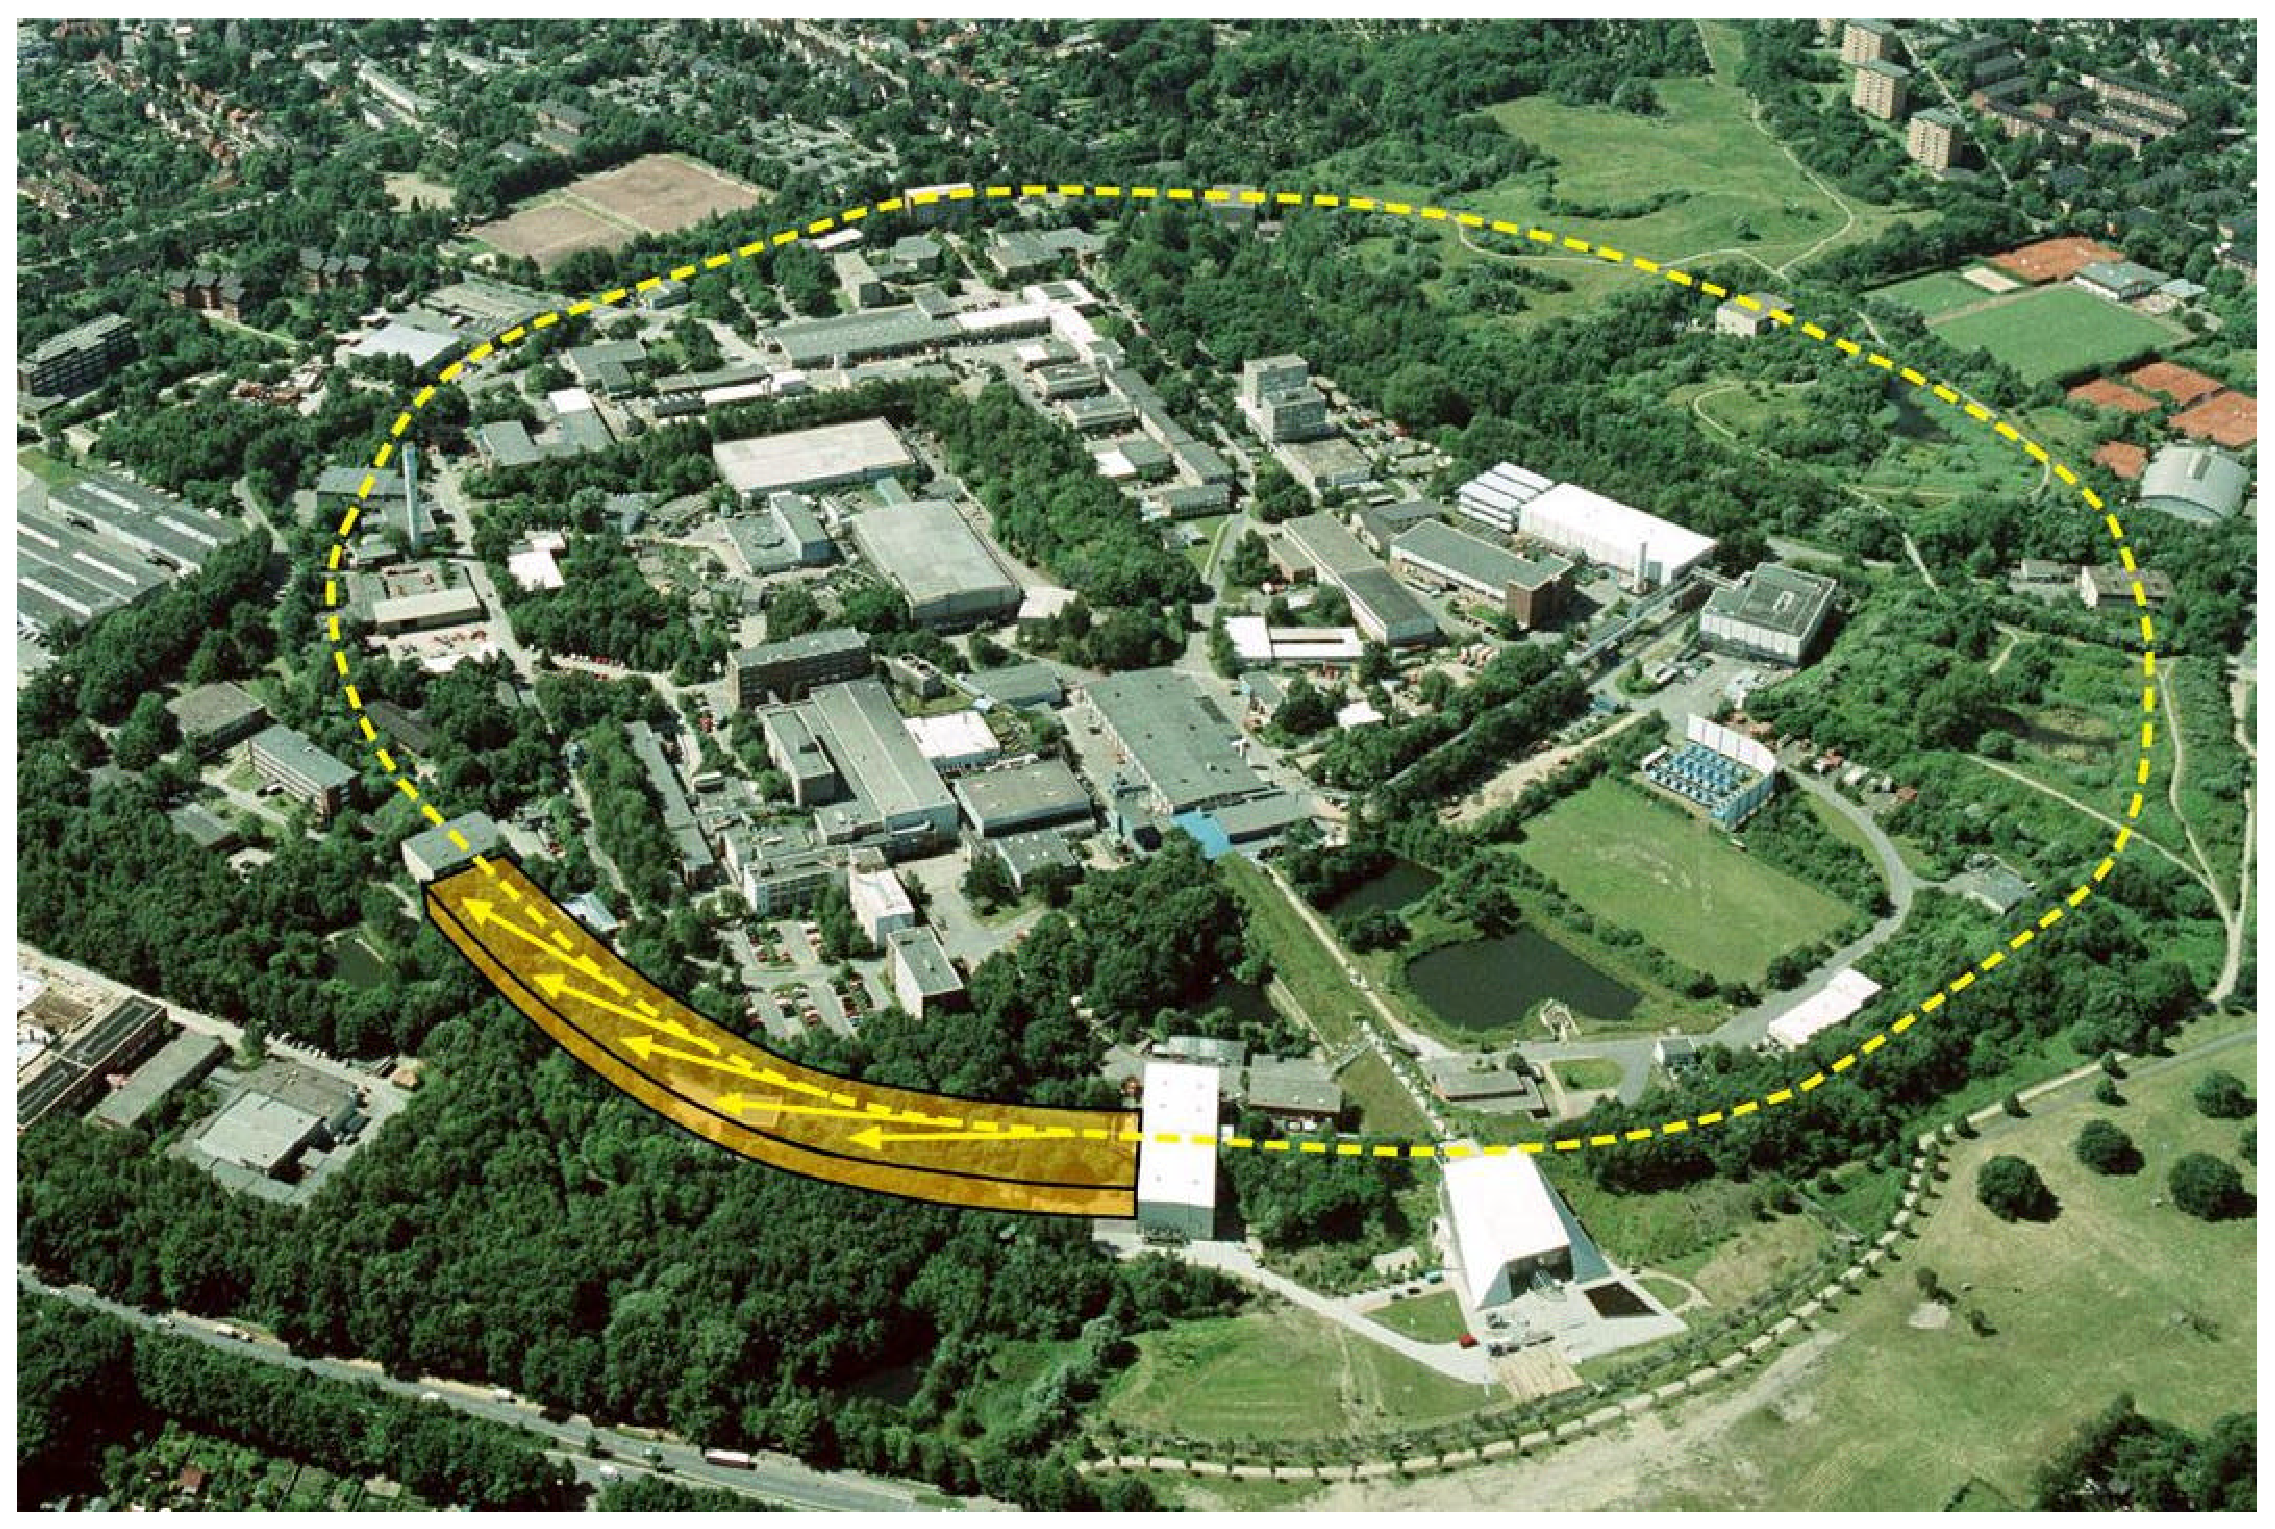
\includegraphics[height=1.0\paperheight,width=\paperwidth]{PETRA}};
}


\frame{\frametitle{JADE  and data preservation}
\begin{columns}[c]
\column{0.54\linewidth}
JADE@PETRA reminder:
\begin{itemize}
\item One of key experiments for QCD: discovery of gluon, $\alpha_{s}$ measurements.
%{\bf 
\item {\bf  The oldest and  most successful  Data Preservation effort!}
\end{itemize}
Motivation for data preservation:
\begin{itemize}
\item Future data (re-)analysis with new models and new approaches.
\item Modelling for the future experiments.
%\item Outreach and education.
%\item {\bf Exceptional example of preservation of 30y.o. data.}
\end{itemize}
\column{0.45\linewidth}
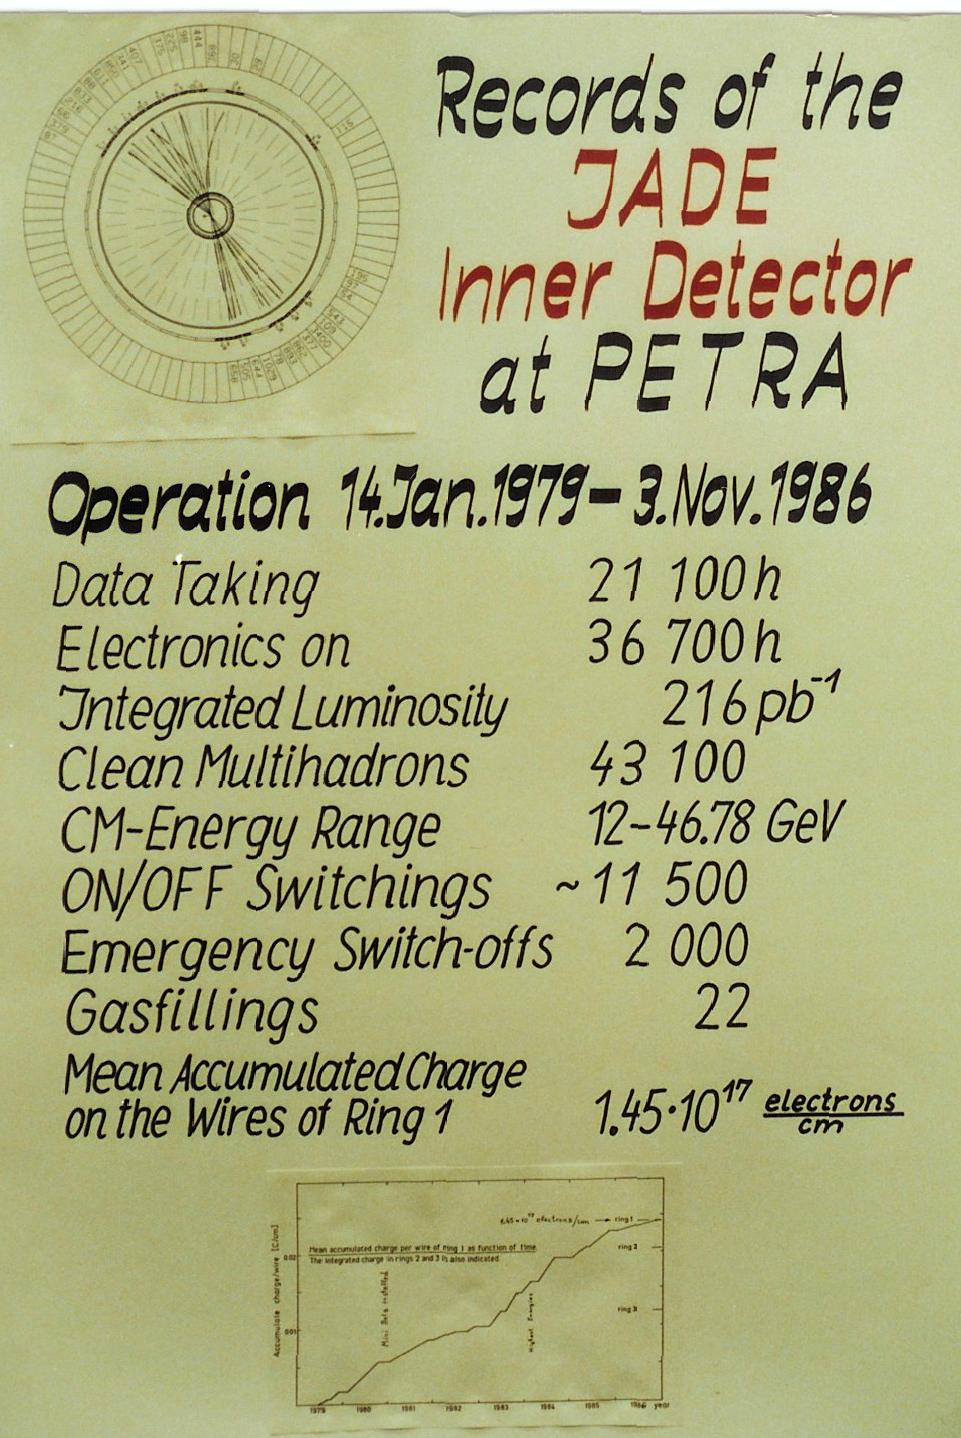
\includegraphics[width=1.0\linewidth]{eps/JADE-ID-records.eps}
\end{columns}
}

\usebackgroundtemplate{}

\frame{\frametitle{JADE data preservation history}
\begin{itemize}
\item 1986: End of data taking.
\item 1995: Private initiative to rescue data (J.~Olsson)
%\begin{itemize}
%\item  rescue data from tapes and copy them to Exabyte cartridges (J.~Olsson)
%\item  reanalyse data with update LEP-like aproach and  theory
%\item  port  JADE software and enable MC generation
%\end{itemize}
%Credits to J.~Olsson, S.~Bethke and P.~Movilla Fernandez.
%}
\item { 1995-2003: Preservation in MPP
\begin{itemize}
\item Physical transfer of data to MPP;
\item Software port to AIX4.3@IBM RS6000;
\item Interface to Pythia6 and Herwig MC;
\item PAW output;
\item Preservation of paper documentation.
\end{itemize}
%Credits to J.~Olsson, S.~Bethke and P.~Movilla Fernandez.
}
\item {1996-2013: Physics
\begin{itemize}
\item 11 papers, O(40) conference talks, thesis, JADE notes.
%\item 4 JADE internal notes.
\end{itemize}
%Credits to S.~Bethke , O.~Biebel , M.~Blumenstengel , S.~Kluth, J.~Olsson , P.~Movilla Fernandez , C.~Pahl , J.~Schieck. 
}
\item {2016-2017: Update of preservation:
\begin{itemize}
\item Data is available online;
\item Software port to Linux(Mac)@$x86\_64$;
%\item Full port of software to $x86\_64$ (Intel-compatible with  Mac)    GNU toolchain;
\item Virtualisation;
\item Interface to HepMC3 (enables most modern MC generator);
\item ROOT output;
\item Preparation of digital documentation on computing notes.
\end{itemize}
%Done by A.V. 
}
\end{itemize}
}







\frame{\frametitle{MPP DP  model for JADE}
\begin{columns}[c]
	\column{0.6\linewidth}
{\centering \bf \color{red}\Large Yes, 11 papers!}\\
{\bf Data preservation is about  new and interested results with old data.}
%A lot of amazing results was obtainded with preserved data in 1995-2013.\\
{\bf In addition  the Data Preservation  experience with JADE has an extreme importance on itself.}\\
In out model we describe  ingredients and tools:\\
\column{0.4\linewidth}
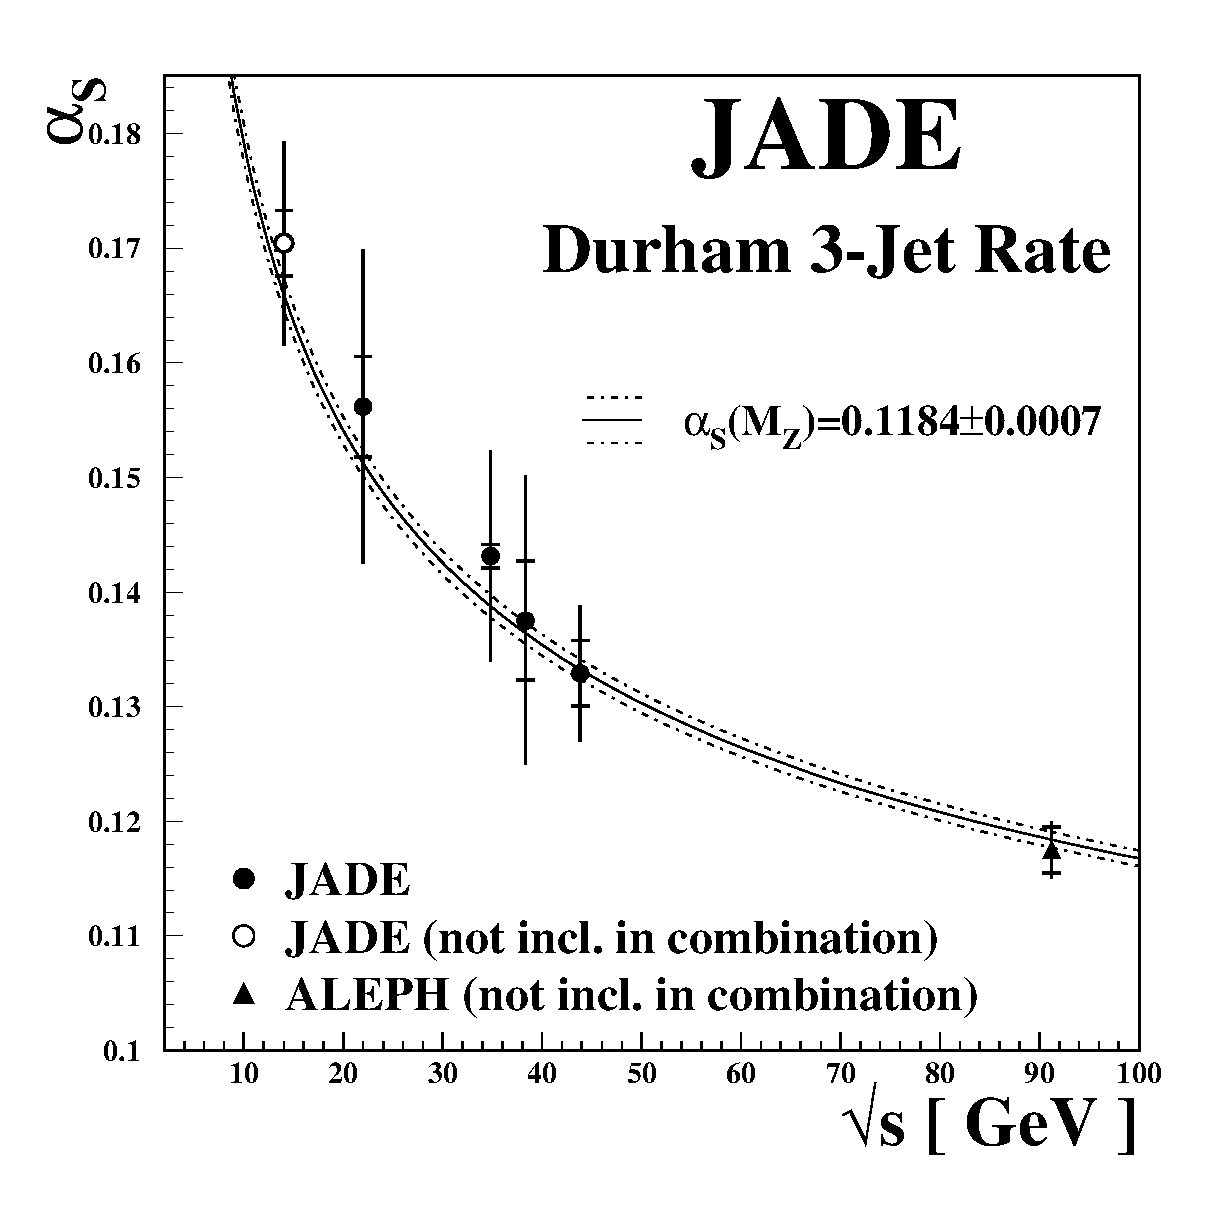
\includegraphics[width=1.0\linewidth,height=0.85\linewidth]{jade_d3_alphas_no14}\\
EPJ C73 (2013) 3, 2332
\end{columns}
\begin{columns}[c]
\column{0.4\linewidth}
\begin{itemize}
\item Data bits
\item Software
\end{itemize}
\column{0.6\linewidth}
\begin{itemize}
\item Experiment documentation
\item DP policies and  documentation
\end{itemize}
\end{columns}

\begin{itemize}
\item But in the end we are interested in {\bf physics }.
\end{itemize}

Main idea: enable physics and make it doable with modern methods in modern environments with minimal effort.\\
}



\frame{\frametitle{MPP DP model for documentation  and policies}
%MPP data preservation relies on the documentation preserved as papers by DESY/DESY library/InSpire.\\
\begin{itemize}
\item JADE publications are available in InSpire, journals, arXiv or scanned by KEK.
\item The non-digital documentation is preserved in DESY and MPP.
\item Logbooks included!
\item Some available online as well, see details at https://wwwjade.mpp.mpg.de/
\end{itemize}
\begin{figure}\centering
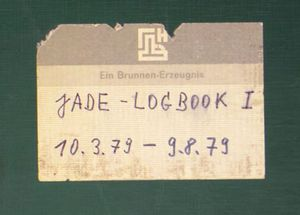
\includegraphics[width=0.3\linewidth]{eps/JADE_Logbook.eps}
\end{figure}
}

\frame{\frametitle{MPP DP model for JADE data bits }
\begin{itemize}
\item JADE data are stored in MPCDF on locally accessible tapes and in disk pool.
\item Access via multiple protocols with grid tools worldwide to disk pools.
%\item Grid-enabled storage for new samples (Monte Carlo) and analysis is available.
\item Straightforward procedure to add new (MC) samples.
\item In the end nowadays all the data from JADE can fit to a modern USB stick.
\end{itemize}
\begin{figure}\centering
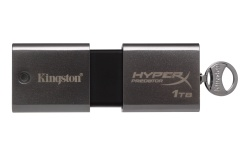
\includegraphics[width=0.25\linewidth]{eps/USB.eps}
\end{figure}
}


%\footnote{Because of data reshiffling now H1 data temporary is only on tape}	


\frame{\frametitle{JADE data in MPP: Bits statistics}
%\hspace{6cm}
\begin{columns}[c]
\column{0.85\linewidth}
Data are  PAW ntuples, ASCII files and FPACK compressed data.
\begin{table}\centering\bf\begin{tabular}{|c|c|c|}\hline
{\color{maroon}           } & {\color{maroon}   MPCDF     }          \\\hline\hline
{\color{maroon}Files:      }&{\color{maroon}   5.4k  } \\
{\color{maroon}Volume:     }&{\color{maroon}   $600 GB$ ($645\times10^{9}$ bytes)} \\
{\color{maroon}Work area:  }&{\color{maroon}    yes       } \\
{\color{maroon}Access:     }&{\color{maroon}   Worldwide  } \\
{\color{maroon}Protocols: } &{\color{maroon}   Multiple, see list   } \\
{\color{maroon}Auth:      } &{\color{maroon}   Grid certificate } \\\hline
\end{tabular}
\end{table}
\column{0.15\linewidth}
\rotatebox{90}{
\includegraphics[height=0.40\linewidth,width=2.8\linewidth]{eps/MPCDF}}
\end{columns}


Available at:
\begin{itemize}
\item gsidcap://grid-srm.rzg.mpg.de:22128/pnfs/rzg.mpg.de/data/zeus/jade
\item grid-gftp2.rzg.mpg.de 
\item davs://grid-dav.rzg.mpg.de:2880//zeus/jade
\item \dots
\end{itemize}

}





\frame{\frametitle{MPP model for software preservation}
Explicit effort put to make software it work in the next 10-15 years.
Previous efforts and high quality of code made it possible.%  porting  was possible.

Key ideas:
\begin{itemize}
\item Rely on industry, not HEP-only standards.
\item Enable integration and compatibility with new physics software, e.g. data bases and Monte Carlo generators.
%\item ISO image of full operating system relying on Intel $x86$  architecture to assure easy usage.
\item {\bf i.e.\ make software analysis-ready}
\end{itemize}


}






\frame{\frametitle{JADE software in MPP}
\begin{itemize}
\item Full chain for reconstruction of raw data to PAW/ROOT ntuples was resurrected.
\item Main software for the analysis of early preserved and reconstructed data is vanilla PAW or ROOT(via h2root).
\item Additional software includes:
\begin{itemize}
\item event display;
\item Monte-Carlo generation packages;
\end{itemize}
\end{itemize}
(Original)Software is available at https://wwwjade.mpp.mpg.de
}




%\frame{\frametitle{JADE software porting quest}
%Source codes were written in  Fortran IV (1974), Fortran 77, Sheltran, Mortran,
  %Assembler.
%Later these were ported to IBM xlf fortran.  

%The original OS/hardware  was UNKNOWN for  on IBM/370 (offline) and Nord 10S/50  (online).
%Later  it became AIX 4.3 on RS6000.


%}

\frame{\frametitle{JADE software porting quest in detail}
\begin{columns}[c]
\column{0.4\linewidth}
\begin{itemize}
\item Original sources in FORTRAN IV (1974), FORTRAN 77, Sheltran, Mortran,
   Assembler ported in 2003 to AIX4.3@RS6000, the old routines replaced with CERNLIB libraries
    and compiled with IBM FORTRAN.\\ {\bf \Large \color{red} Huge work!}
\end{itemize}
\column{0.6\linewidth}
\begin{figure}\centering
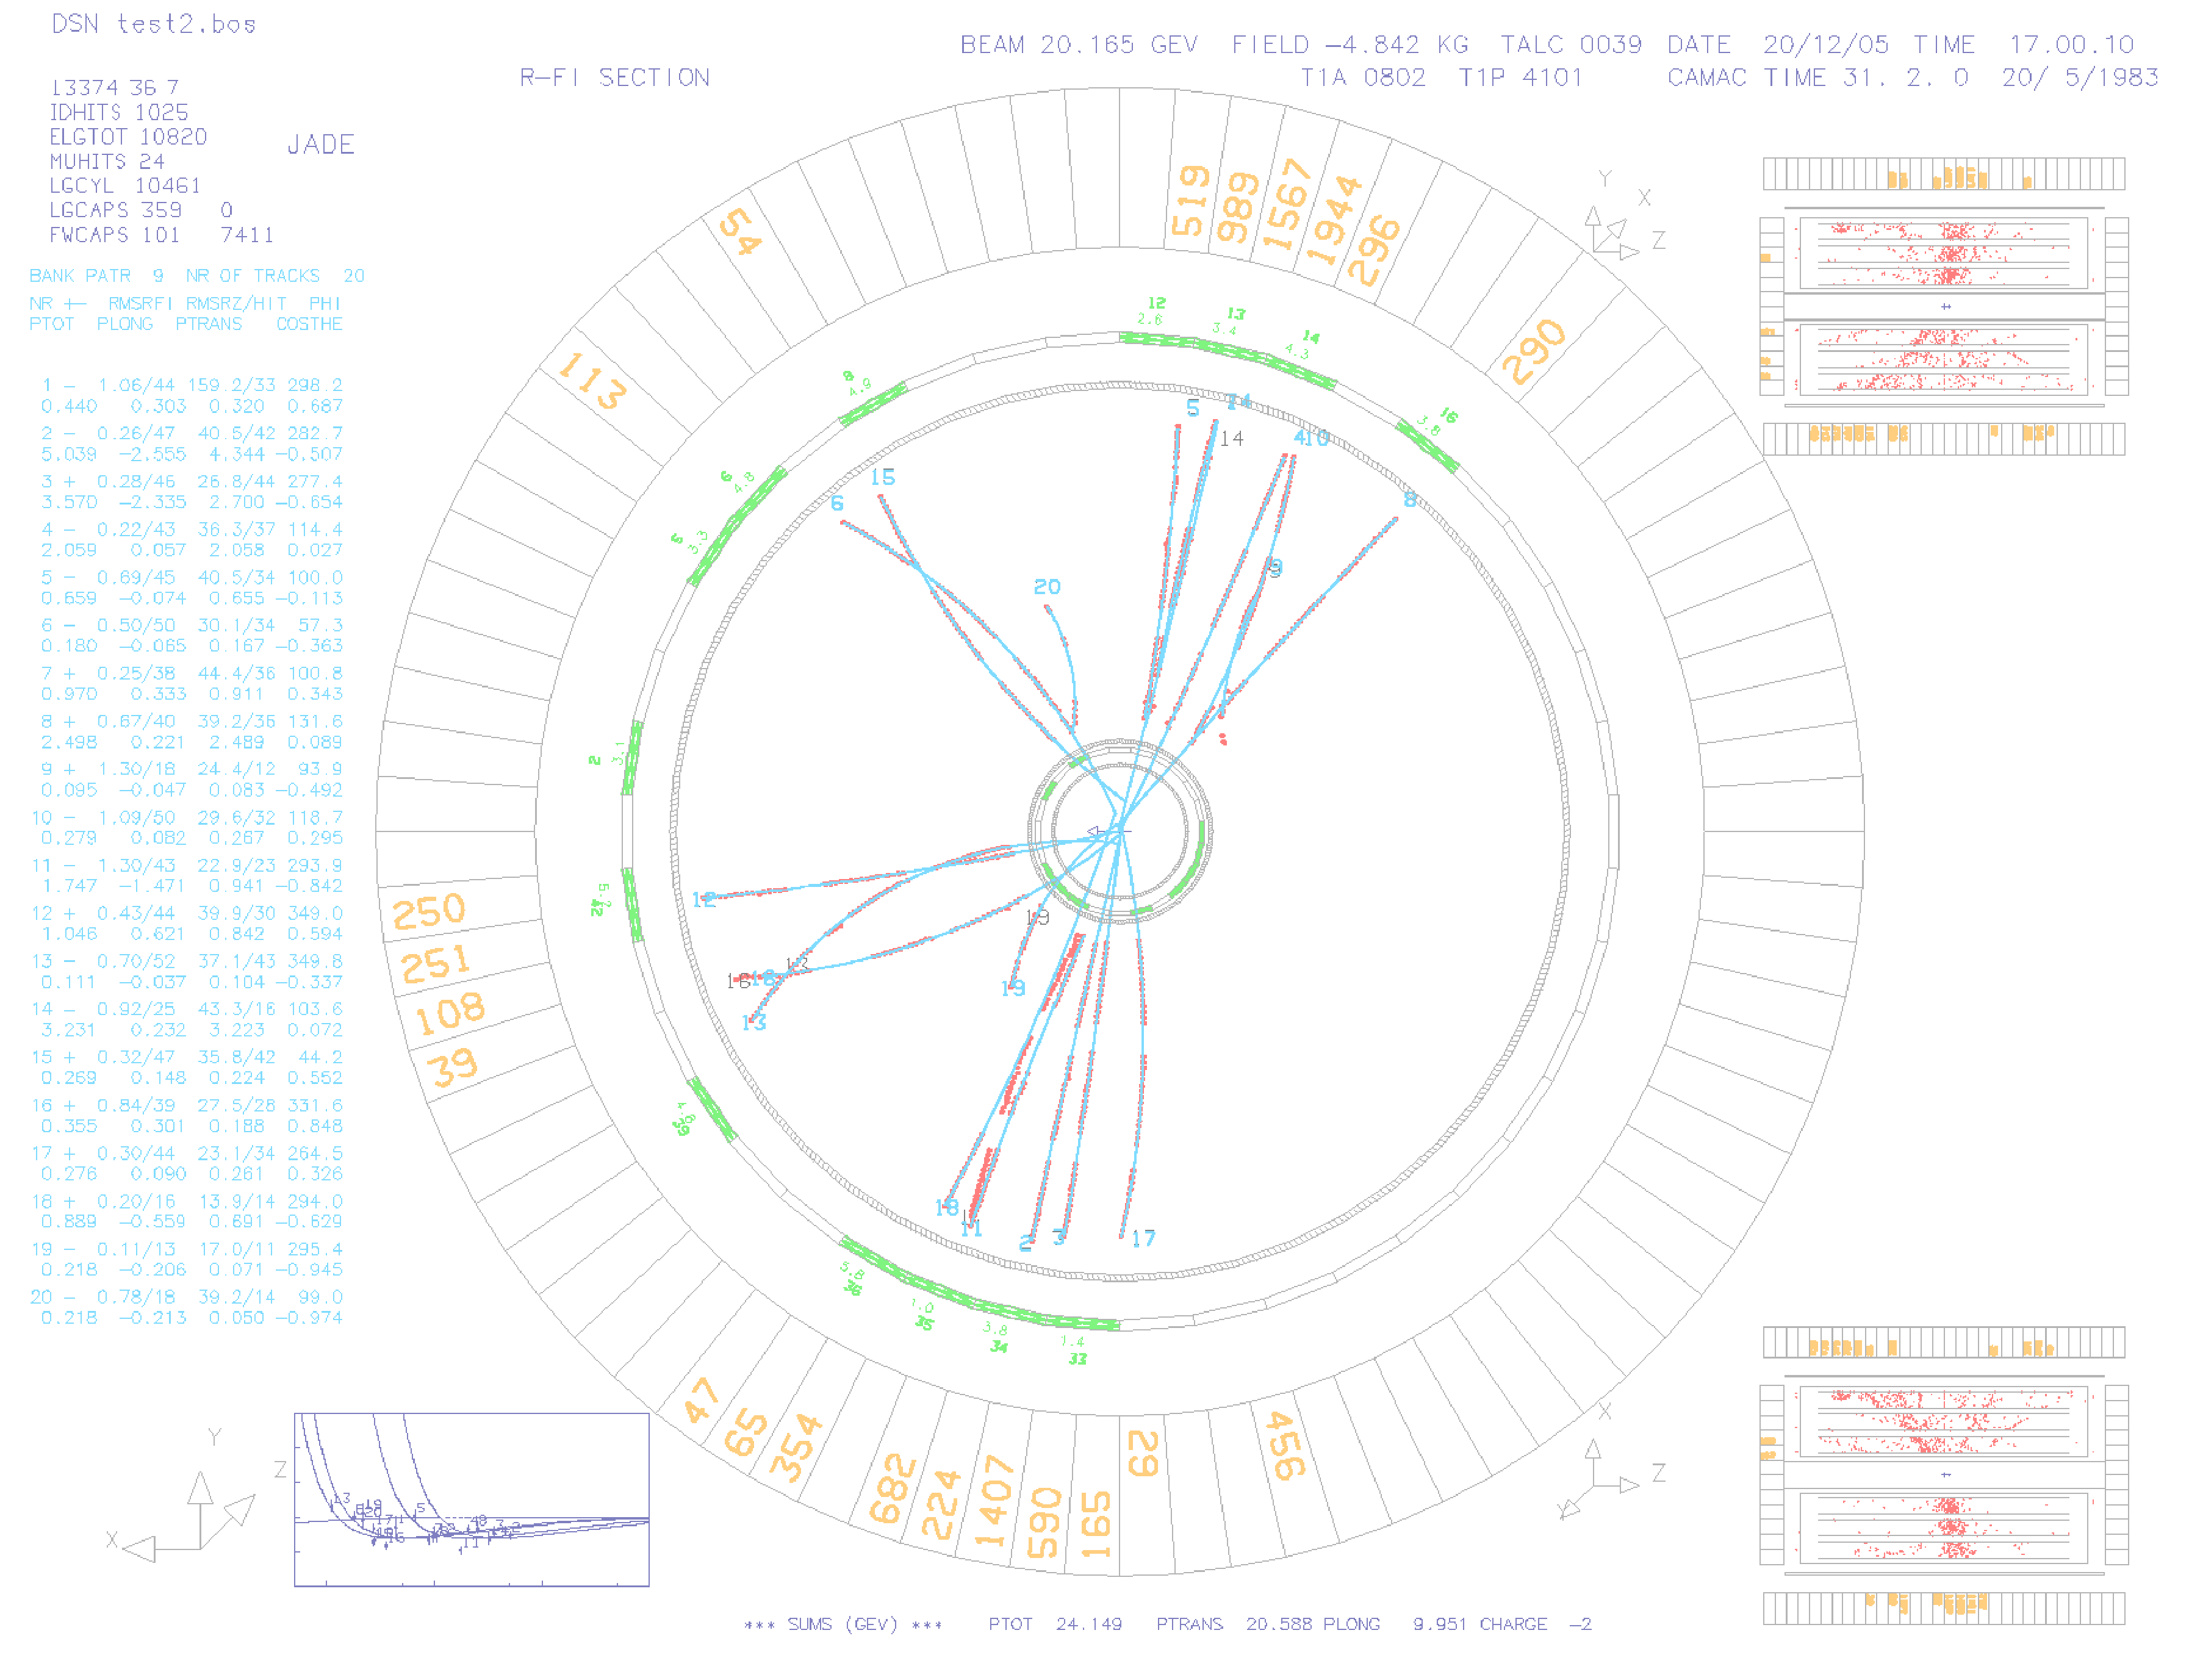
\includegraphics[width=1.0\linewidth]{jadedisplayold.eps}
\end{figure}
\end{columns}
\begin{itemize}
\item In 2017 everything is problematic: AIX@ppc is Big Endian architecture, no CERNLIB in modern systems,
IBM FORTRAN is not for free, 32 bit systems are dying out etc.
\end{itemize}
}



\frame{\frametitle{JADE software porting quest: step one}
One can start from:
\begin{itemize}
\item 	PowerPC64 multi-arch CentOS7 Big Endian on QEMU2.7;
\item   CERNLIB compilation for PowerPC {\bf \color{red} Yes, for many flavours!};
\item   Trial version of IBM xlf15 for Linux;
\item   Manual or semiautomatic fixes of differences between FORTRAN dialects (e.g. HOLLERITH, INTEGER vs. CHARECTER).
\end{itemize}

FYI: Some codes date back to 1974.
}

\frame{\frametitle{JADE software porting quest: step two}
Once the software passes simplest tests:
\begin{itemize}
\item 	Switch to gfortran;
\item   Start to use cmake (best thing for FORTRAN!);
\item   Switch to Little Endian Linux and control I/O Endianess with GFORTRAN\_CONVERT\_UNIT ;
\item   Replace as many as possible CERNLIB routines with ROOT or dummy routines;
\item   The remaining routines just copy from CERNLIB (i.e. create "picocernlib");
\item   {\bf \color{red}Compile codes in native 64-bit mode.}

\end{itemize}


}


\frame{\frametitle{JADE software porting quest: step two}
Once the code is compiled on a standard computer, one has to fix bugs in functionality or implement missing features.\\ 
Here the problems begin.
\begin{itemize}
\item 	Part of the code was lost long time ago: muon reconstruction is not available.
\item   Event display was ported to HIGZ/CERNLIB in 2003. To the version of CERNLIB that is hard to find.
Most graphics primitives re-implemented in ROOT, but display is still not fully operational.
\item   The data is compressed with FPACK utility, but the way it was done is not known, same as the way to unpack it.
A collaboration with J.Olsson might be helpful.
\end{itemize}


}


\frame{\frametitle{JADE software porting quest: step three}
On the positive site:
\begin{itemize}
\item The key to productive usage of JADE data in the past was an option to generate MC with much newer generators.
The option was implemented with integration of Pythia/Herwig/Ariadne codes into JADE software.
\item Now it is simpler: Monte Carlo generators have standard output formats and only a converter from a standard format to JADE-specific input has to be developed.
\item Done with HepMC3, very nice library.
\end{itemize}


}




%\frame{\frametitle{JADE software porting quest: step one}
%After downloading the tarbal with software from 2003:


%One has to find big endian machine, something RS6000 (ppc) compatible.

%Solution is QEMU2.7 virtual machine with ppc/ppc64 support. 
%Another option, old  RS6000 machine used as router turns out to be slow and has not enough disk space.
%RS6000 are availbale on e-bay, but are quite expensive.


%One has to find modern big endian OS, something AIX43 compatible.
%Solution is CentOS7.2 with multiarch support ppc64+ppc(64be+32be) from CentOS AltArch repository. 

%One has to find xlf compatible compiler.
%Solution is a trial version of xlf 15.1 from IBM.
%Thanks, IBM!

%Now we can try to compile something!
%}

%\frame{\frametitle{JADE software porting quest: step one}

%One has to have a build system for the software. Old makefiles are impractical.
%Solution is the new cmake. cmake is PERFECT for fortran. 


%The fortran dialect incompatibilities are fixed by hand or with sed scripts. 
%These are mostly HOLLERITHs, INTEGER to CHARECTER conversion and so on.
%Takes some time, but is a straightforward procedure.
%{\bf At this point everything compiles. }

%One has to link programs with some CERNLIB routines.
%Subquest: compile 32 bit CERNLIB for CentOS7 on ppc.
%With some tricks 32 bit CERNLIB rpm package was obtained. 
%See explanations in the backup.

%{\bf At this point executables are linked and tested.}
%At the next step gfortran was used to compile the executables.
%{\bf At this point  the stup is complitely open source.}
%Next, the CentOS7 x8664 with multiach support wasused instead of the  ppc version.
%The byteorder issues are solved with gfortran runtime which accepts big endian byteorder I/O if to set a proper environment variable.
%export GFORTRAN\_CONVERT\_UNIT='big\_endian;native:2' 
%The CERNLIB was compiled for this planform as well.

%{\bf At this point  the setup can be used on many standard machines, only 32 bit libraries and  CERNLIB is required.}

%}


%\frame{\frametitle{JADE software porting quest: step one}

%CERNLIB is not supported, so it is a good idea to throw it away.
%The main dependence on cernlib are  just few generic routines and HIGZ package for graphics.

%The generic routines were copied from cernlib and the graphic primitives were replaced with ROOT 
%drawing routines. The small set of routines was collected to form  "picocernlib".% can be compiled even in 64 bit mode.

%{\bf At this point  the setup can be used on many standard machines, only ROOT is required.}




%}




\frame{\frametitle{JADE software environment/VM}
A certain environment is needed  for the analysis.
\begin{itemize}
\item Virtual machines(VM) are a very attractive {\bf long-term} solution;
\item The way other experiments (LEP/LHC) are going;
\item The solution has very generic requirements, will survive for a long time.
\item Unlimited number of installations $\rightarrow$ potentially usable on clouds;
\item Usage not restricted to any laboratory or virtualisation software. Can run anywhere.
\item Usage of ISO installation image assures vendor independence.
\end{itemize}
VM is available at: https://wwwjade.mpp.mpg.de
}




\usebackgroundtemplate{}


\frame{\frametitle{JADE software environment/VM}
VM includes:
\begin{itemize}
\item JADE software: ROOT, MC simulation, event display, file catalogue, setup scripts etc. See a detailed list in backup slides.
\item Modern MC generators, FastJet, CERNLIB, PAW and other popular and ``not really'' packages.
\item Anything you will want to install\dots
%\item Available at: https://wwwJADE.mpp.mpg.de/dphep.html together with  documentation and video tutorials. 
\item Agree access and download it.
\item VirtualBox images are provided as well.
\end{itemize}
}



\frame{\frametitle{JADE software environment/VM}
\begin{figure}\centering
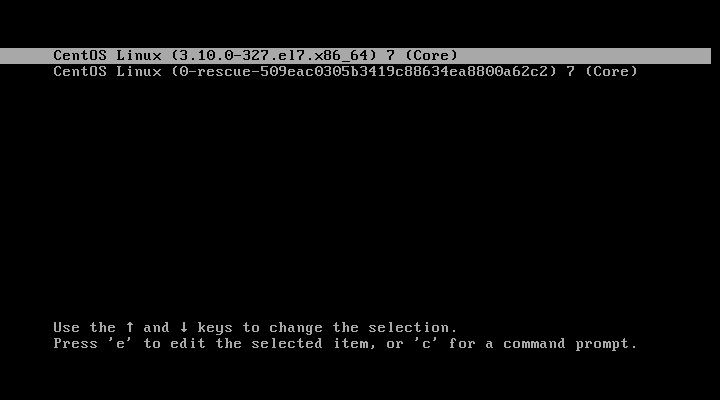
\includegraphics[width=0.75\textwidth]{eps/start.eps}
\end{figure}
Generic start of VM.
}


\frame{\frametitle{JADE software environment/VM test }
\begin{figure}\centering
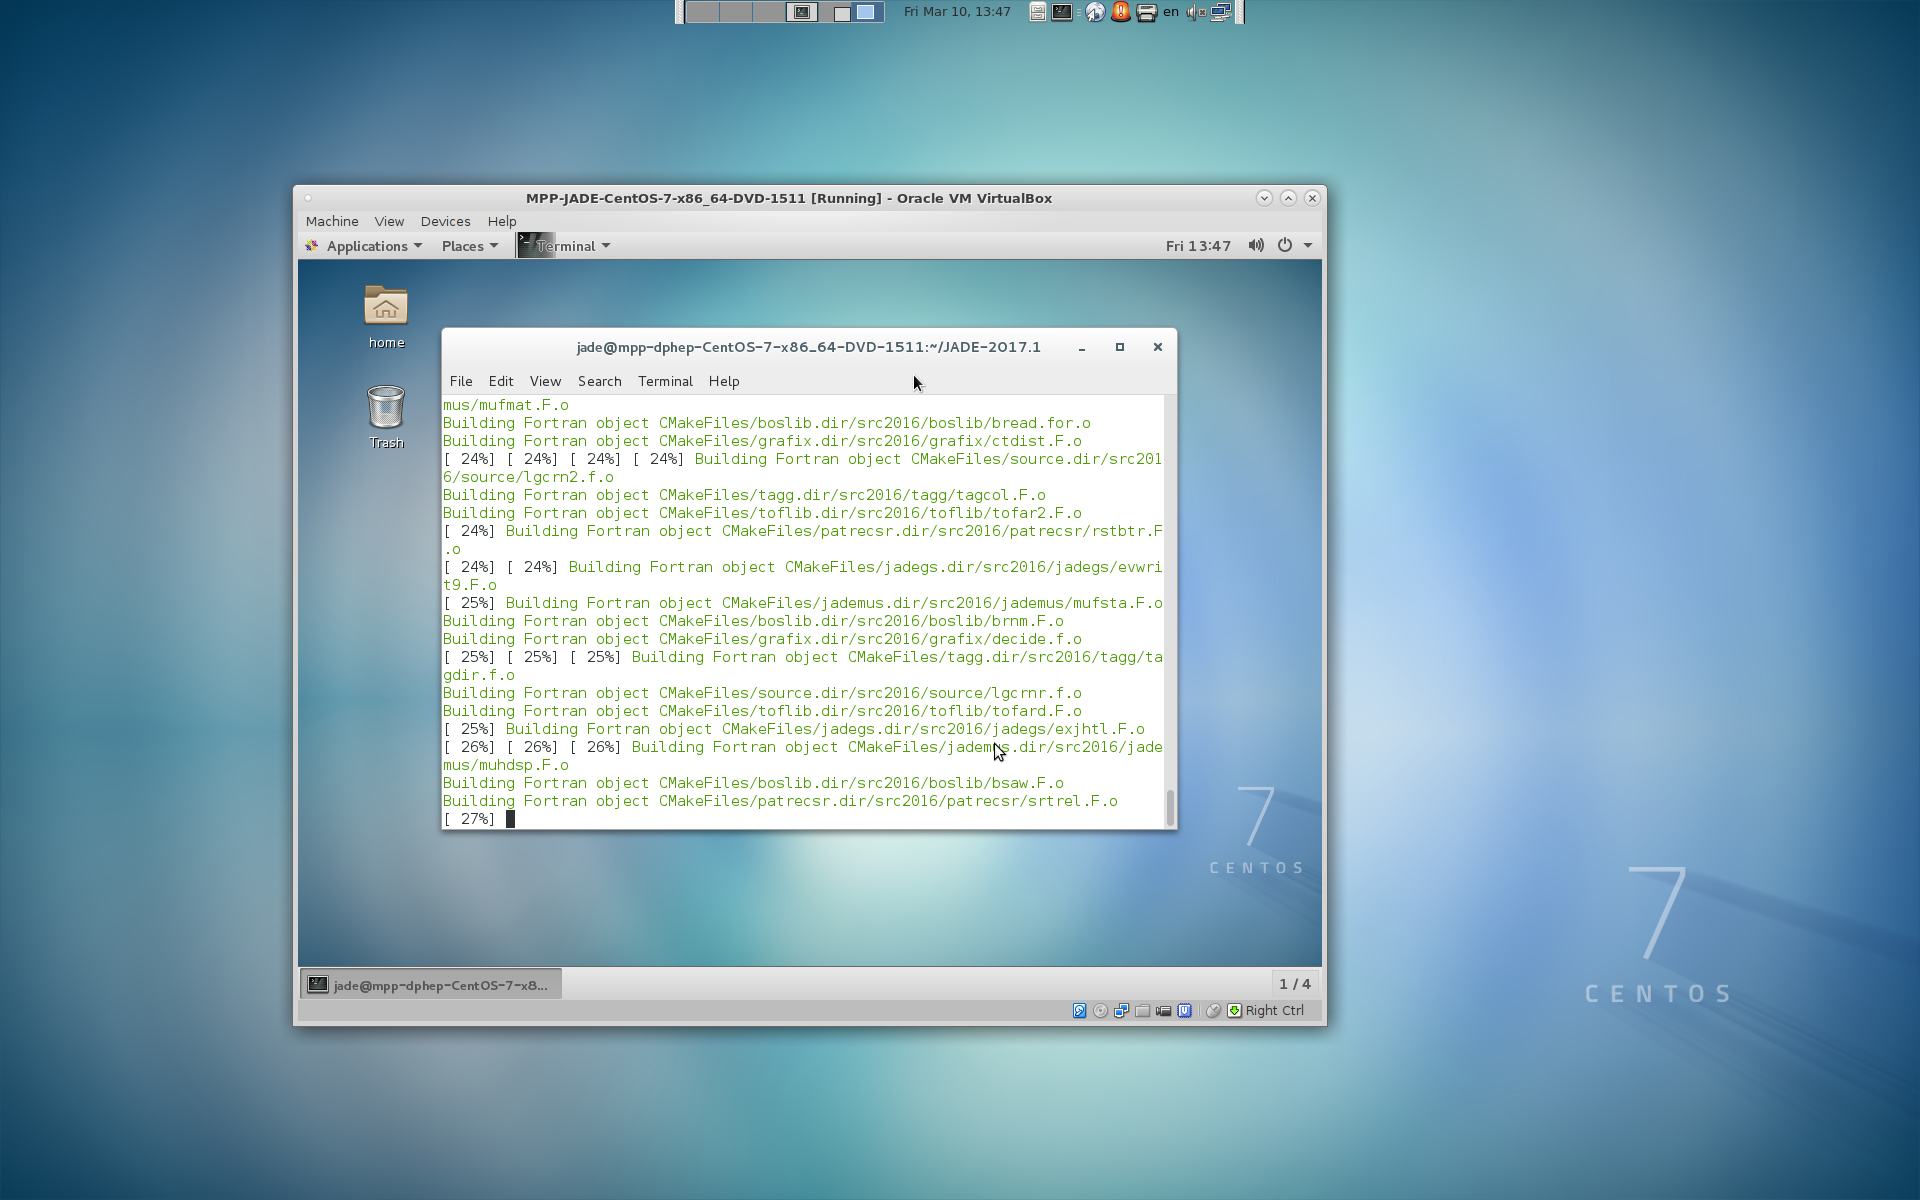
\includegraphics[width=0.75\textwidth]{eps/compilation.eps}
\end{figure}
JADE software compilation in VM: takes about 4 minutes.
}


\frame{\frametitle{JADE software environment/VM test }
\begin{figure}\centering
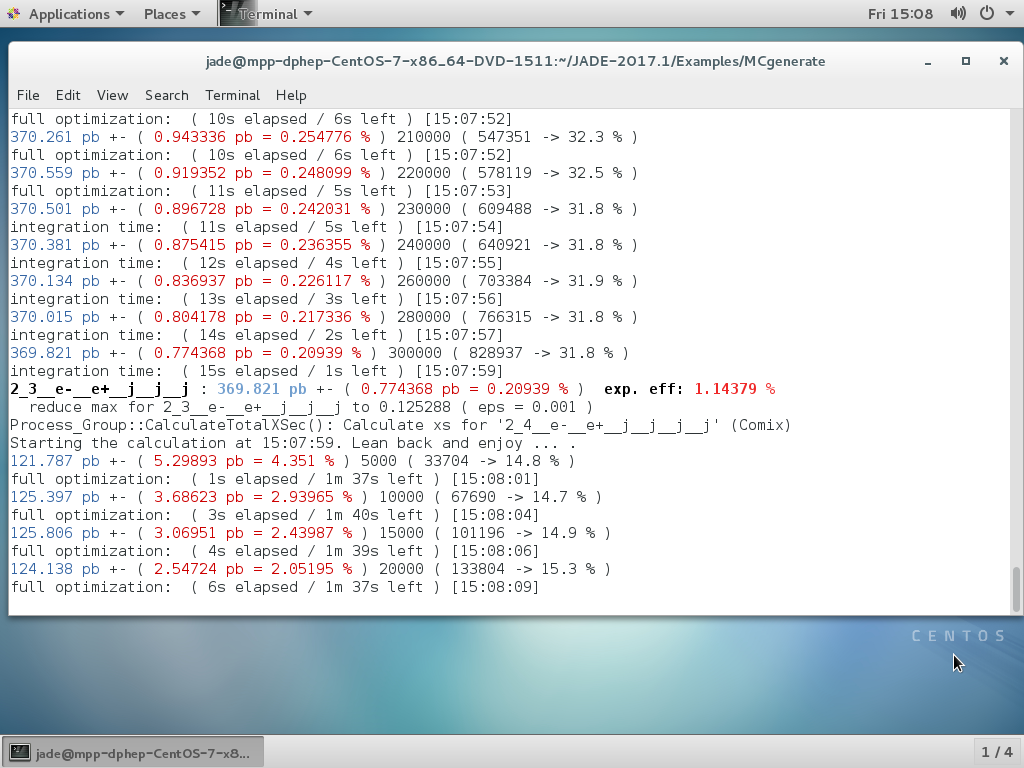
\includegraphics[width=0.75\textwidth]{eps/sherpa.eps}
\end{figure}
MC for JADE can be generated in VM or elsewhere. In this case SHERPA is running in VM.
}


\frame{\frametitle{JADE software environment/VM test }
\begin{figure}\centering
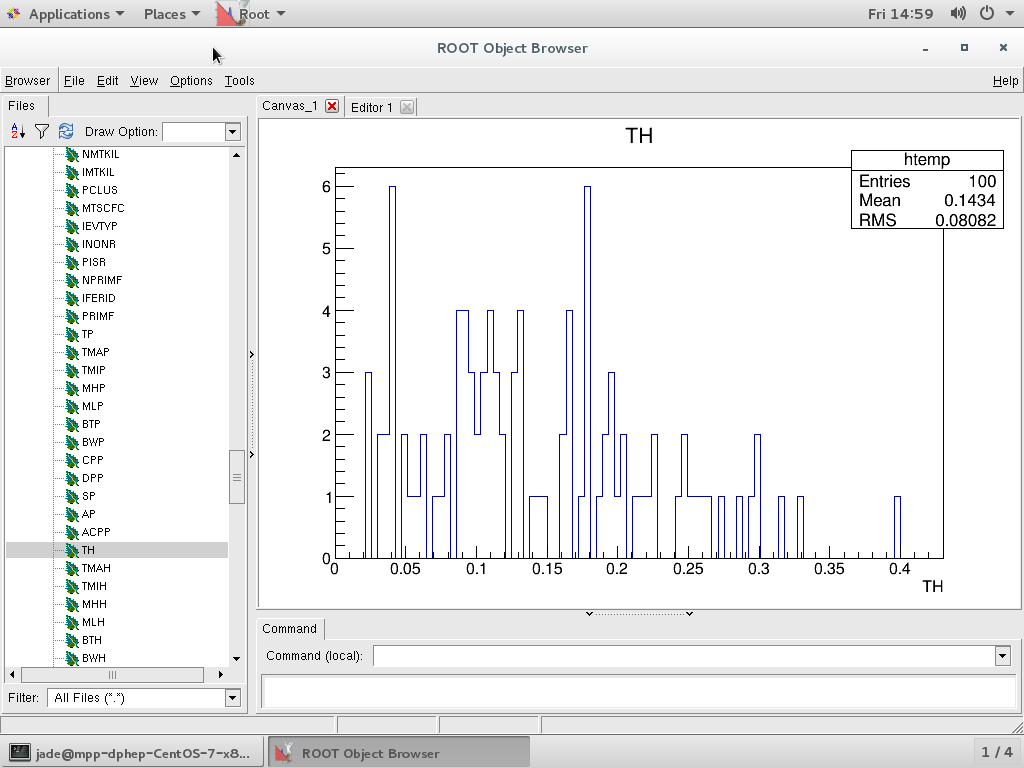
\includegraphics[width=0.75\textwidth]{eps/thrust.eps}
\end{figure}
In the end of reconstruction a ROOT file with simple tree is delivered.  %Reconstruction takes fractions of second even in VM. 
Thrust distribution from the generated evens is shown.
}

\frame{\frametitle{JADE software environment/VM test }
\begin{figure}\centering
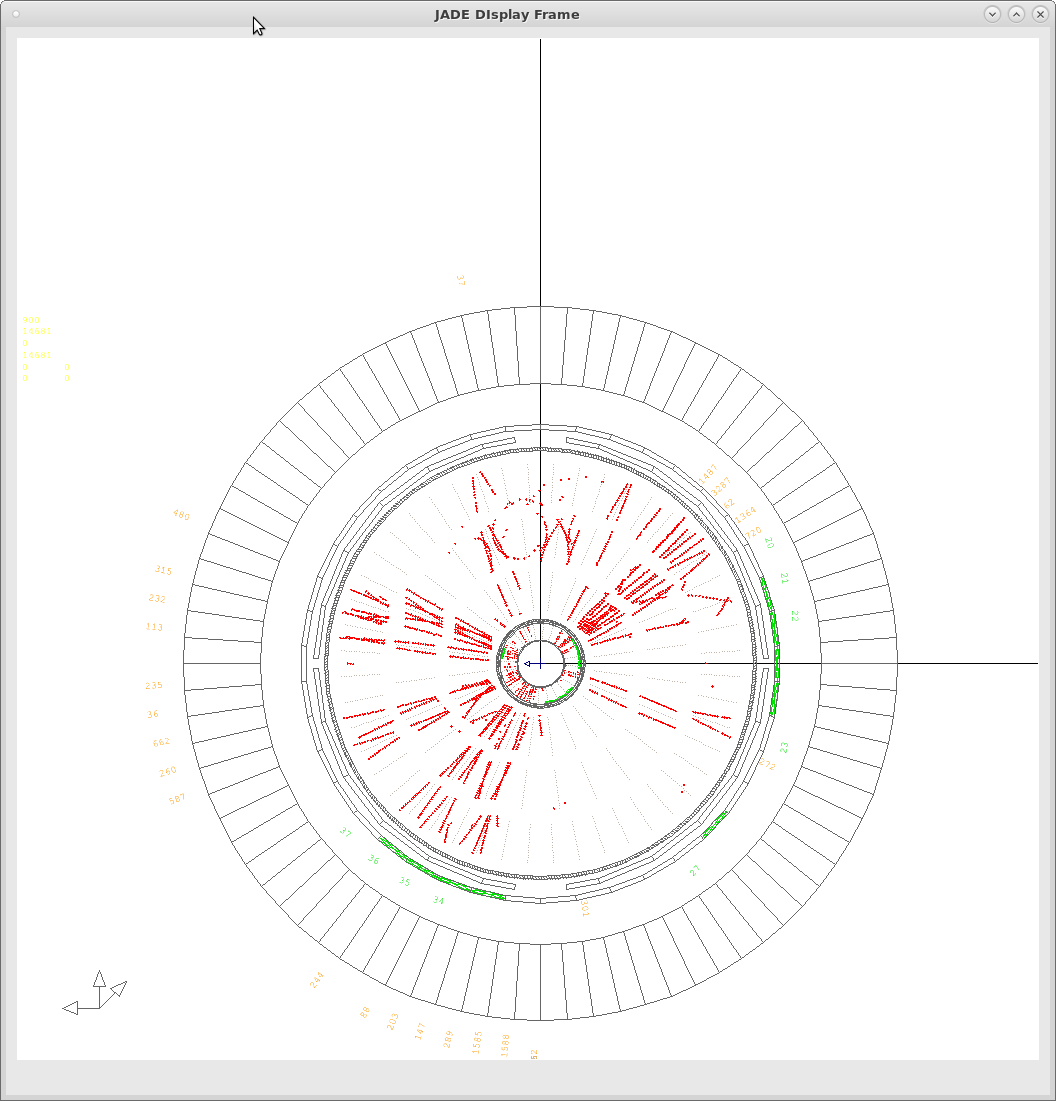
\includegraphics[width=0.55\textwidth]{eps/jadezroot.eps}
\end{figure}
Test of the reconstructed MC files with event display.
{\bf Not all functionality is restored. To be fixed.}.
}






\section{Conclusions}

\frame{\frametitle{MPP Data Preservation summary}
\begin{itemize}
\item Huge work was done since 1995!
\item Many high quality, important physics results delivered.
\item Data is accessible in  MPCDF and software is {\bf\color{red}analysis-ready}.
%\item An option for MC production with new and old MC generators exists for JADE and tested. 
%\item Existing data ntuples can be used with generated MC samples, i.e. {\bf system is analysis-ready}.
\end{itemize}
Potential improvements are obvious: enable data reading, fixes to event display, improving documentation.
}
\section{Data Preservation applications}
\frame{\frametitle{JADE Data Preservation applications}
\begin{itemize}
\item Hadronisation effects.
\item QCD with $b$-quarks and modern theory predictions, e.g. tests of future fully differential NNLO predictions for $e^{+}e^{-}\rightarrow hadrons$ with heavy quarks.
\item \dots
\end{itemize}
}


\frame{\frametitle{}}

\section{What other experiments can learn from JADE DP}


\frame{\frametitle{Software}
\begin{itemize}
\item Generic technologies for hardware and OS is an advantage.
\item High code quality, clarity and stability is a key to success.
Note: some routines are from 1974, i.e. 43 y.o. 
Few modern experiments can be sure that more than tiny fraction of their code will behave like that.
\item Design of software is important.%, even complicated things like event display can survive for 30 years if to use good simple approaches, i.e. graphic primitives in this case.
\item Good build system makes porting much easier
\item Standardisation of I/O data formats is important.
\item Documentation on simple things is important, i.e. meaning of arguments for utilities.
\end{itemize}
}

\frame{\frametitle{Data}

\begin{itemize}
\item Compressing the data might look like a good solution, but it is bad. Saving 1Tb of disk space today mean lose of days to read the data back tomorrow.
{\color{red} Do not compress your data!}
\item Keeping reference data/MC/results is important.
\item Standardisation of I/O data formats is important.
\end{itemize}
}



\frame{\frametitle{What other experiments can learn from JADE DP: Some anecdotes}
\begin{itemize}
\item one "calibration" file, with  luminosities for each run and fill, was stored on a private account  and therefore lost when DESY archive was cleaned up;
\item   Jan Olsson, when cleaning up his office in ~1997, found an old ASCII-printout of the JADE luminosity file.
  Unfortunately, it was printed on green recycling paper - not suitable for scanning and OCR-ing.
  A secretary at Aachen re-typed it within 4 weeks.
  A checksum routine found (and recovered) only 4 typos.
\item an old version of the original BOSlib 1979 version was found, on  request at the Tokyo computer centre.
\item  Peter Bock, when cleaning out an old lab at the Physics Institute at Heidelberg University, found a few 9-track tapes containing 
original JADE MC files which were very valuable for validating
  results of first re-analyses in ~1997
\end{itemize}
}

\frame{\frametitle{What other experiments can learn from JADE DP: Some anecdotes}
\begin{itemize}
\item First port attempt in 2016 was done with AIX 4.3 machine used as router in MPP, but turns out VirtualBox is more useful.
\item Many problems in software porting were solved in the industry: byte ordering problem  in the modern gfortran, availability of 
Linux on PowerPCs, good FORTRAN build system (cmake) is available now, xlf compiler is available on Linux now.
\item Googling the arxiver used fro the data, FPACK is a hard task.
\end{itemize}


%best computer in 19985 is 2GFLOPS, CRAY2   1 core now 45GFLOPS

}
\frame{\frametitle{List of custom/extra RPM packages on JADE VM}
Some subpackages omitted.

\begin{columns}[c]\tiny
\column{0.5\linewidth}
blackhat-0.9.9-1.el7.centos.x86\_64.rpm
blas-devel-3.4.2-5.el7.x86\_64.rpm
cernlib-2006-36.el7.centos.i686.rpm
cernlib-devel-2006-36.el7.centos.i686.rpm
cernlib-packlib-gfortran-2006-36.el7.centos.i686.rpm
cernlib-static-2006-36.el7.centos.i686.rpm
cernlib-utils-2006-36.el7.centos.i686.rpm
epel-release-7-5.noarch.rpm
fastjet-3.1.2-1.el7.centos.x86\_64.rpm
form-4.1-1.el7.centos.x86\_64.rpm
geant321-2006-36.el7.centos.i686.rpm
gosam-2.0.3-1.el7.centos.x86\_64.rpm
gosam-contrib-2.0-1.el7.centos.x86\_64.rpm
Herwig-7.0.2-2.el7.centos.x86\_64.rpm
lapack-devel-3.4.2-5.el7.x86\_64.rpm
\column{0.5\linewidth}
LHAPDF-6.1.6-6.el7.centos.x86\_64.rpm
osg-ca-certs-1.55-1.el7.centos.noarch.rpm
osg-release-3.3-5.el7.centos.noarch.rpm
patchy-gfortran-2006-36.el7.centos.i686.rpm
paw-gfortran-2006-36.el7.centos.i686.rpm
PHOTOS-3.61-1.el7.centos.x86\_64.rpm
pythia8-8.2.15-102.el7.centos.x86\_64.rpm
qd-2.3.15-100.el7.centos.x86\_64.rpm
qgraf-3.1.4-1.el7.centos.x86\_64.rpm
root-5.34.36-1.el7.centos.x86\_64.rpm
SHERPA-MC-2.2.0-3.el7.centos.x86\_64.rpm
TAUOLA-1.1.5-1.el7.centos.x86\_64.rpm
ThePEG-2.0.2-1.el7.centos.x86\_64.rpm
vincia-1.2.02-1.el7.centos.x86\_64.rpm
xbae-4.60.4-12.el7.centos.i686.rpm
\end{columns}

All JADE software is packed as one rpm that is installed as is in /opt
}
\end{document}

